\bta{测定电源的电动势和内阻}

\begin{enumerate}[leftmargin=0em]
\renewcommand{\labelenumi}{\arabic{enumi}.}
% A(\Alph) a(\alph) I(\Roman) i(\roman) 1(\arabic)
%设定全局标号series=example	%引用全局变量resume=example
%[topsep=-0.3em,parsep=-0.3em,itemsep=-0.3em,partopsep=-0.3em]
%可使用leftmargin调整列表环境左边的空白长度 [leftmargin=0em]
\item
\exwhere{$ 2016 $年北京卷}
某兴趣小组探究用不同方法测定干电池的电动势和内阻,他们提出的实验方案中有如下四种器材组合。为使实验结果尽可能准确,最不可取的一组器材是 \xzanswer{D} 

\fourchoices
{一个安培表、一个伏特表和一个滑动变阻器}
{一个伏特表和多个定值电阻}
{一个安培表和一个电阻箱}
{两个安培表和一个滑动变阻器}

\item 
\exwhere{$ 2013 $年浙江卷}
采用如图所示的电路“测定电池的电动势和内阻”。
\begin{figure}[h!]
\centering
\includesvg[width=0.53\linewidth]{picture/svg/693}
\end{figure}

\begin{enumerate}
\renewcommand{\labelenumi}{\arabic{enumi}.}
% A(\Alph) a(\alph) I(\Roman) i(\roman) 1(\arabic)
%设定全局标号series=example	%引用全局变量resume=example
%[topsep=-0.3em,parsep=-0.3em,itemsep=-0.3em,partopsep=-0.3em]
%可使用leftmargin调整列表环境左边的空白长度 [leftmargin=0em]
\item
除了选用图中的部分器材外, \tk{A} 
(填选项)
\fourchoices
{还需要电压表}
{还需要电流表}
{还需要学生电源}
{不再需要任何器材}

\item 
测量所得数据如下:


\begin{table}[h!]
\centering 
\begin{tabular}{|c|c|c|c|c|c|c|}
\hline 
\diagbox{测量次数}{物理量} & 1 & 2 & 3 & 4 & 5 & 6
\\
\hline
R/$ \Omega $& 1.2 & 1.0 & 0.8 & 0.6 & 0.4 & 0.2
\\
\hline
I/A & 0.60 & 0.70 & 0.80 & 0.89 & 1.00 & 1.20
\\
\hline
U/V & 0.90 & 0.78 & 0.74 & 0.67 & 0.62 & 0.43\\ 
\hline 
\end{tabular}
\end{table} 

用作图法求得电池的内阻$ r= $ \tk{$ (0.75\pm 0.10)\ \Omega $} 
;

\item 
根据第$ 5 $组所测得的实验数据,求得电流表内阻$ R_{A} = $ \tk{0.22 $\Omega$} 
。



\end{enumerate}

\newpage


\item 
\exwhere{$ 2016 $年四川卷}
用如图所示电路测量电源的电动势和内阻。实验器材:待测电源(电动势约$ 3 $ $ V $,内阻约$ 2 $ $ \Omega $),保护电阻$ R_{1} $(阻值$ 10 $ $ \Omega $)和$ R_{2} $(阻值$ 5 $ $ \Omega $),滑动变阻器$ R $,电流表$ A $,电压表$ V $,开关$ S $,导线若干。
\begin{figure}[h!]
\centering
\includesvg[width=0.23\linewidth]{picture/svg/692}
\end{figure}

实验主要步骤:

($ i $)将滑动变阻器接入电路的阻值调到最大,闭合开关;

($ ii $)逐渐减小滑动变阻器接入电路的阻值,记下电压表的示数$ U $和相应电流表的示数 $ I $ ;

($ iii $)以$ U $为纵坐标, \lmd{1} 为横坐标,作$ U-I $ 图线($ U $、 $ I $ 都用国际单位);

($ iv $)求出$ U-I $ 图线斜率的绝对值$ k $和在横轴上的截距$ a $。

回答下列问题:

\begin{enumerate}
\renewcommand{\labelenumi}{\arabic{enumi}.}
% A(\Alph) a(\alph) I(\Roman) i(\roman) 1(\arabic)
%设定全局标号series=example	%引用全局变量resume=example
%[topsep=-0.3em,parsep=-0.3em,itemsep=-0.3em,partopsep=-0.3em]
%可使用leftmargin调整列表环境左边的空白长度 [leftmargin=0em]
\item
电压表最好选用 \tk{A} 
;电流表最好选用 \tk{C} 
。
\fourchoices
{电压表($ 0 \sim 3 $ $ V $,内阻约$ 15 $ $ k \Omega $)}
{电压表($ 0 \sim 3 $ $ V $,内阻约$ 3 $ $ k \Omega $)}
{电流表($ 0 \sim 200 $ $ m{A} $,内阻约$ 2 $ $ \Omega $)}
{电流表($ 0 \sim 30 $ $ m{A} $,内阻约$ 2 $ $ \Omega $)}

\item 
滑动变阻器的滑片从左向右滑动,发现电压表示数增大。两导线与滑动变阻器接线柱连接情况是 \tk{C} 
。
\fourchoices
{两导线接在滑动变阻器电阻丝两端接线柱}
{两导线接在滑动变阻器金属杆两端接线柱}
{一条导线接在滑动变阻器金属杆左端接线柱,另一条导线接在电阻丝左端接线柱}
{一条导线接在滑动变阻器金属杆右端接线柱,另一条导线接在电阻丝右端接线柱}

\item 
选用$ k $、$ a $、$ R_{1} $和$ R_{2} $表示待测电源的电动势$ E $和内阻$ r $的表达式$ E= $ \tk{$ ka $} 
,$ r= $ \tk{$ k-R_{2} $} 
,代入数值可得$ E $和$ r $的测量值。





\end{enumerate}






\newpage
\item 
\exwhere{$ 2013 $年安徽卷}
根据闭合电路欧姆定律,用图$ 1 $所示电路可以测定电池的电动势和内电阻。图中$ R _ 0 $是定值电阻,通过改变$ R $的阻值,测出$ R $ $ 0 $两端的对应电压$ U_{1} 2 $,对所得的实验数据进行处理,就可以实现测量目的。根据实验数据在$\frac { 1 } { U _ { 12 } } - R$坐标系中描出坐标点,如图$ 2 $所示。已知$R _ { 0 } = 150 \Omega$,请完成以下数据分析和处理。
\begin{figure}[h!]
\centering
\includesvg[width=0.73\linewidth]{picture/svg/694}
\end{figure}


\begin{enumerate}
\renewcommand{\labelenumi}{\arabic{enumi}.}
% A(\Alph) a(\alph) I(\Roman) i(\roman) 1(\arabic)
%设定全局标号series=example	%引用全局变量resume=example
%[topsep=-0.3em,parsep=-0.3em,itemsep=-0.3em,partopsep=-0.3em]
%可使用leftmargin调整列表环境左边的空白长度 [leftmargin=0em]
\item
图$ 2 $中电阻为 \tk{80.0} 
$ \Omega $的数据点应剔除;
\item 
在坐标纸上画出$\frac { 1 } { U _ { 12 } } - R $关系图线;
\item 
图线的斜率是 \tk{0.00444} 
,由此可得电池电动势$ E_x= $ \tk{1.50} 
$ V $。



\end{enumerate}


\banswer{
(2)如图示 :
 \includesvg[width=0.23\linewidth]{picture/svg/695} 
}



\item
\exwhere{$ 2011 $年理综四川卷}
为测量一电源的电动势及内阻:

①在下列三个电压表中选一个改装成量程为$ 9V $的电压表

\threechoices
{量程为$ 1\ V $、内阻大约为$ 1 \ k\Omega $的电压表 
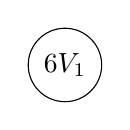
\begin{tikzpicture}[baseline=-0.4em]
\node[draw,circle] (4,0) {\zihao{6}$ V_{1} $};
\end{tikzpicture}
}
{量程为$ 2\ V $、内阻大约为$ 2 \ k\Omega $的电压表
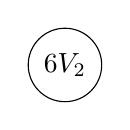
\begin{tikzpicture}[baseline=-0.4em]
\node[draw,circle] (4,0) {\zihao{6}$ V_{2} $};
\end{tikzpicture}
}
{量程为$ 3\ V $、内阻为$ 3 \ k\Omega $的电压表
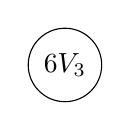
\begin{tikzpicture}[baseline=-0.4em]
\node[draw,circle] (4,0) {\zihao{6}$ V_{3} $};
\end{tikzpicture}
}

选择电压表 \tk{C} 
串联 \tk{6} 
$ k \Omega $的电阻可以改装成量程为$ 9\ V $的电压表。 

②利用一个电阻箱、一只开关、若干导线和改装好的电压表(此表用符号
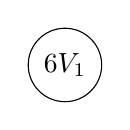
\begin{tikzpicture}[baseline=-0.4em]
\node[draw,circle] (4,0) {\zihao{6}$ V_{1} $};
\end{tikzpicture}
、
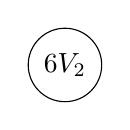
\begin{tikzpicture}[baseline=-0.4em]
\node[draw,circle] (4,0) {\zihao{6}$ V_{2} $};
\end{tikzpicture}
或
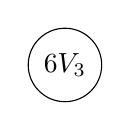
\begin{tikzpicture}[baseline=-0.4em]
\node[draw,circle] (4,0) {\zihao{6}$ V_{3} $};
\end{tikzpicture}
与一个电阻串联来表示,且可视为理想电压表),在虚线框内画出测量电源电动势及内阻的实验原理电路图。
\begin{figure}[h!]
\centering
\includesvg[width=0.23\linewidth]{picture/svg/701}
\end{figure}



③根据以上实验原理电路图进行实验,读出电压表示数为$ 1.50V $时、电阻箱的阻值为$ 15.0 \ \Omega $,电压表示数为$ 2.00V $时,电阻箱的阻值为$ 40.0 \ \Omega $,则电源的电动势$ E= $ \tk{7.5} 
$ V $、内阻$ r= $ \tk{10} 
$ \Omega $。 


\banswer{
②实验原理电路图如图示。
\includesvg[width=0.23\linewidth]{picture/svg/702} 
}


\newpage

\item 
\exwhere{$ 2012 $年理综四川卷}
某学习小组的同学拟探究小灯泡$ L $的伏安特性曲线,可供选用的器材如下:

小灯泡$ L $,规格“$ 4.0V $.$ 0.7A $”;

电流表$ A_{1} $,量程$ 3A $,内阻约为$ 0.1 \ \Omega $; 

电流表$ A_{2} $,量程$ 0.6A $,内阻$ r_{2} =0.2 \ \Omega $;

电压表$ V $,量程$ 3V $,内阻$ rV=9 \ k\Omega $; 

标准电阻$ R_{1} $,阻值$ 1 \ \Omega $;

标准电阻$ R_{2} $,阻值$ 3 $ $ k \Omega $;

滑动变阻器$ R $,阻值范围$ 0 \sim $ $ 10 \ \Omega $;

学生电源$ E $,电动势$ 6V $,内阻不计;

开关$ S $及导线若干。

①甲同学设计了如图$ 1 $所示的电路来进行测量,当通过$ L $的电流为$ 0.46\ A $时,电压表的示数如图$ 2 $所示,此时$ L $的电阻为 \tk{5} 
$ \Omega $。
\begin{figure}[h!]
\centering
\includesvg[width=0.2\linewidth]{picture/svg/696} \qquad \includesvg[width=0.2\linewidth]{picture/svg/697} \qquad \includesvg[width=0.2\linewidth]{picture/svg/698} \qquad \includesvg[width=0.2\linewidth]{picture/svg/699} 
\end{figure}

②乙同学又设计了如图$ 3 $所示的电路来进行测量,电压表指针指在最大刻度时,加在$ L $上的电压值是 \tk{4} 
$ V $。

③学习小组认为要想更准确地描绘出$ L $完整的伏安特性曲线,需要重新设计电路。请你在乙同学的基础上利用所供器材,在图$ 4 $所示的虚线框内补画出实验电路图,并在图上标明所选器材代号。


\banswer{
③由于电压表量程太小,所以需要改装,将它与$ R_{2} $串联即成为一个量程为$ 4.0V $的新的电压表;电流表$ A_{1} $量程太大,不可用,可以将$ A_{2} $改装:将它并联一个小电阻$ R_{1} $则成为一个量程为$ 0.72A $的新的电流表了。由于灯泡的电阻远小于电压表内阻而与电流表内阻相差不多,属于小电阻,故用电流表外接法比较合适。答案如答图$ 1 $较合适,若用答图$ 2 $则不太合适。

 \includesvg[width=0.4\linewidth]{picture/svg/700} 
 
说明:画出答图$ 1 $给$ 4 $分,只画出答图$ 2 $给$ 2 $分。
}




\newpage
\item
\exwhere{$ 2012 $年理综福建卷}
某研究性学习小组欲测定一块电池的电动势$ E $。

①先直接用多用电表测定该电池电动势。在操作无误的情况下,多用电表表盘示数如图,其示数为 \tk{9.4} 
$ V $。
\begin{figure}[h!]
\centering
\includesvg[width=0.23\linewidth]{picture/svg/703}
\end{figure}

②然后,用电压表$ V $、电阻箱$ R $、定值电阻$ R_{0} $、开关$ S $、若干导线和该电池组成电路,测定该电池电动势。
\begin{figure}[h!]
\centering
\includesvg[width=0.83\linewidth]{picture/svg/704}\\
 \begin{tabular}{|c|c|c|c|c|c|c|}
\hline 
R ($ \Omega $) & 166.7 & 71.4 & 50.0 & 33.3 & 25.0 & 20.0
\\
\hline
U (V) & 8.3 & 5.9 & 4.8 & 4.2 & 3.2 & 2.9
\\
\hline
$1/R
( \times 10^{-2} \Omega ^{-1}) $ & 0.60 & 1.40 & 2.00 & 3.00 & 4.00 & 5.00
\\
\hline
$ 1/U(V^{0} ) $ & 0.12 & 0.17 & 0.21 & 0.24 & 0.31 & 0.35\\ 
\hline 
\end{tabular}
\end{figure}




\begin{enumerate}
\renewcommand{\labelenumi}{\arabic{enumi}.}
% A(\Alph) a(\alph) I(\Roman) i(\roman) 1(\arabic)
%设定全局标号series=example	%引用全局变量resume=example
%[topsep=-0.3em,parsep=-0.3em,itemsep=-0.3em,partopsep=-0.3em]
%可使用leftmargin调整列表环境左边的空白长度 [leftmargin=0em]
\item
根据电路图,用笔画线代替导线,将实物图连接成完整电路。
\item 
闭合开关$ S $,调整电阻箱阻值$ R $,读出电压表$ V $相应示数$ U $。该学习小组测出大量数据,分析筛选出下表所示的$ R $、$ U $数据,并计算出相应的$ 1/R $与$ 1/U $的值。请用表中数据在坐标纸上描点,并作出$ 1/U-1/R $图线。

\item 
从图线中可以求得电动势$ E=$ \tk{$ 9.5-11.1 $} 
$V $	

\end{enumerate}


\banswer{
(ⅰ)连接电路如图所示。
(ⅱ)所作图象如图所示
 \includesvg[width=0.23\linewidth]{picture/svg/705} 
}



\newpage
\item 
\exwhere{$ 2018 $年江苏卷}
一同学测量某干电池的电动势和内阻。

\begin{enumerate}
\renewcommand{\labelenumi}{\arabic{enumi}.}
% A(\Alph) a(\alph) I(\Roman) i(\roman) 1(\arabic)
%设定全局标号series=example	%引用全局变量resume=example
%[topsep=-0.3em,parsep=-0.3em,itemsep=-0.3em,partopsep=-0.3em]
%可使用leftmargin调整列表环境左边的空白长度 [leftmargin=0em]
\item
如图所示是该同学正准备接入最后一根导线(图中虚线所示)时的实验电路。请指出图中在器材操作上存在的两个不妥之处。
\begin{figure}[h!]
\centering
\includesvg[width=0.23\linewidth]{picture/svg/706}
\end{figure}

 \tk{①开关未断开 ②电阻箱阻值为零}\hfullline 


\item 
实验测得的电阻箱阻值$ R $和电流表示数 $ I $ ,以及计算的$ \frac{1}{I} $数据见下表:
\begin{table}[h!]
\centering 
\begin{tabular}{|c|c|c|c|c|c|}
\hline 
R/$ \Omega $ & 8.0 & 7.0 & 6.0 & 5.0 & 4.0
\\
\hline
I/A & 0.15 & 0.17 & 0.19 & 0.22 & 0.26
\\
\hline
$ \frac{1}{I}/A^{–1} $ & 6.7 & 6.0 & 5.3 & 4.5 & 3.8\\ 
\hline 
\end{tabular}
\end{table} 

根据表中数据,在答题卡的方格纸上作出$R - \frac { 1 } { I }$关系图象。由图象可计算出该干电池的电动势为 \tk{$ 1.4 $($ 1.30 \sim 1.44 $都算对)} 
$ V $;内阻为 \tk{$ 1.2 $($ 1.0 \sim 1.4 $都算对)} 
$ \Omega $。
\begin{figure}[h!]
\centering
\includesvg[width=0.53\linewidth]{picture/svg/707}
\end{figure}


\item 
为了得到更准确的测量结果,在测出上述数据后,该同学将一只量程为$ 100 $ $ mV $的电压表并联在电流表的两端。调节电阻箱,当电流表的示数为$ 0.33 $ $ A $时,电压表的指针位置如图$ 2 $所示,则该干电池的电动势应为 \tk{$ 1.4 $(结果与($ 2 $)问第一个空格一致)} 
$ V $;内阻应为 \tk{$ 1.0 $(结果比($ 2 $)问第二个空格小$ 0.2 $)} 
$ \Omega $。



\end{enumerate}


\banswer{
($ 2 $)(见下图) :
 \includesvg[width=0.23\linewidth]{picture/svg/708} 
}


\newpage
\item 
\exwhere{$ 2014 $年理综新课标\lmd{1}卷}
利用如图$ (a) $所示电路,可以测量电源的电动势和内阻,所用的实验器材有:
待测电源,电阻箱$ R $(最大阻值$ 999.9 $ $ \Omega ) $,电阻$ R_{0} $(阻值为$ 3.0 $ $ \Omega ) $,电阻$ R_{1} $(阻值为$ 3.0 $ $ \Omega ) $,电流表$ A $(量程为$ 200 $ $ m{A} $,内阻为$ R_{A} =6.0 $ $ \Omega ) $,开关$ S $. 
\begin{figure}[h!]
\centering
\includesvg[width=0.23\linewidth]{picture/svg/709} \qquad 
 \includesvg[width=0.23\linewidth]{picture/svg/710} \qquad 
 \includesvg[width=0.23\linewidth]{picture/svg/711} 
\end{figure}



实验步骤如下:

①将电阻箱阻值调到最大,闭合开关$ S $;

②多次调节电阻箱,记下电流表的示数$ I $ 和电阻值箱相应的阻值$ R $;

③以$ \frac{1}{I} $为纵坐标,$ R $为横坐标,作 ­$\frac { 1 } { I } - R$ 图线(用直线拟合);

④求出直线的斜率$ k $和在纵轴上的截距$ b $. 为 \underlinegap .

回答下列问题:
\begin{enumerate}
\renewcommand{\labelenumii}{(\arabic{enumii})}
\item 
分别用$ E $和$ r $表示电源的电动势和内阻,则 与$ R $的关系式为$\frac { 1 } { I } = \frac { R _ { A } + R _ { 1 } } { E R _ { 1 } } R + \frac { 1 } { E } \left[ R _ { A } + \frac { R _ { A } + R _ { 1 } } { R _ { 1 } } \left( R _ { 0 } + r \right) \right]$.


\item 
实验得到的部分数据如下表所示,其中电阻$ R=3.0 $ $ \Omega $时电流表的示数如图$ (b) $所示,读出数据,完成下表.答:① \tk{0.110} 
,② \tk{9.09} 
.
\begin{table}[h!]
\centering 
\begin{tabular}{|c|c|c|c|c|c|c|c|}
\hline 
R/$ \Omega $ & 1.0 & 2.0 & 3.0 & 4.0 & 5.0 & 6.0 & 7.0
\\
\hline
I/A & 0.143 & 0.125 & ① & 0.100 & 0.091 & 0.084 & 0.077
\\
\hline
$ I^{-1}/A^{-1} $ & 6.99 & 8.00 & ② & 10.0 & 11.0 & 11.9 & 13.0\\ 
\hline 
\end{tabular}
\end{table} 


\item 
在图$ (c) $的坐标纸上将所缺数据点补充完整并作图,根据图线求得斜率$ k= $ \tk{1.0(在$ 0.961.04 $之间均给分) } 
$A^{-1} \Omega^{ -1} $,截距$ b= $ \tk{6.0(在$ 5.9\sim 6.1 $之间均给分)} 
$A^{-1} $.


\item 
根据图线求得电源电动势$ E=$ \tk{3.0 V (在$ 2.7\sim 3.3 $之间均给分)} 
$V $,内阻$ r= $ \tk{$1.0 \ \Omega $(在$ 0.6\sim 1.4 $之间均给分)} 
$\Omega $. 

\end{enumerate}

\banswer{
(3)图线如答图 
 \includesvg[width=0.23\linewidth]{picture/svg/712} 
}


\newpage
\item 
\exwhere{$ 2014 $年理综大纲卷}
现要测量某电源的电动势和内阻。可利用的器材有:电流表 \ammetermytikz ,内阻为$ 1.00 \ \Omega $;电压表 \voltmetermytikz ;阻值未知的定值电阻$ R_{1} $、$ R_{2} $、$ R_{3} $、$ R_{4} $、$ R_{5} $;开关$ S $;一端连有鳄鱼夹$ P $的导线$ 1 $,其他导线若干。某同学设计的测量电路如图$ (a) $所示。
\begin{figure}[h!]
\centering
\includesvg[width=0.83\linewidth]{picture/svg/713}
\end{figure}



\begin{enumerate}
\renewcommand{\labelenumi}{\arabic{enumi}.}
% A(\Alph) a(\alph) I(\Roman) i(\roman) 1(\arabic)
%设定全局标号series=example	%引用全局变量resume=example
%[topsep=-0.3em,parsep=-0.3em,itemsep=-0.3em,partopsep=-0.3em]
%可使用leftmargin调整列表环境左边的空白长度 [leftmargin=0em]
\item
按图 $ (a) $在实物图$ (b) $中画出连线,并标出导线$ 1 $和其$ P $端。
\item 
测量时,改变鳄鱼夹$ P $所夹的位置,使$ R_{1} $、$ R_{2} $、$ R_{3} $、$ R_{4} $、$ R_{5} $依次串入电路,记录对应的电压表的示数$ U $和电流表的示数 \lmd{1} 。 数据如下表所示。根据表中数据,在图($ c $)中的坐标纸上将所缺数据点补充完整,并画出$ U-I $图线。

\begin{figure}[h!]
\centering 
\begin{tabular}{|c|c|c|c|c|c|}
\hline 
I(mA) & 193 & 153 & 111 & 69 & 30
 \\
\hline
U(V) & 2.51 & 2.59 & 2.68 & 2.76 & 2.84\\ 
\hline 
\end{tabular} \qquad 
\includesvg[width=0.35\linewidth]{picture/svg/714} 
\end{figure}


\item 
根据$ U-I $图线求出电源的电动势$ E= $ \tk{$ 2.90 $(在$ 2.89 \sim 2.91 $之间均给分)} 
$ V $,内阻$ r= $ \tk{$ 1.02 $(在$ 0.93 \sim 1.13 $之间均给分)} 
$ \Omega $。




\end{enumerate}

\banswer{
$ (1) $连接如答图$ 1 $所示.$ U $­ \lmd{1} 图线如答图$ 2 $所示.

 \includesvg[width=0.23\linewidth]{picture/svg/715} 
}



\newpage
\item 
\exwhere{$ 2014 $年理综北京卷}
利用电流表和电压表测定一节干电池的电动势和内电阻。要求尽量减小实验误差。
\begin{enumerate}
\renewcommand{\labelenumi}{\arabic{enumi}.}
% A(\Alph) a(\alph) I(\Roman) i(\roman) 1(\arabic)
%设定全局标号series=example	%引用全局变量resume=example
%[topsep=-0.3em,parsep=-0.3em,itemsep=-0.3em,partopsep=-0.3em]
%可使用leftmargin调整列表环境左边的空白长度 [leftmargin=0em]
\item
应该选择的实验电路是图$ 1 $中的 \tk{甲} 
(选项“甲”或“乙”)。
\begin{figure}[h!]
\centering
\includesvg[width=0.37\linewidth]{picture/svg/716}
\end{figure}

\item 
现有电流表($ 0\sim 0.6\ A $)、开关和导线若干,以及以下器材:
\fourchoices
{电压表($ 015V $)}
{电压表($ 03V $)}
{滑动变阻器($ 050 \ \Omega $)}
{滑动变阻器($ 0500 \ \Omega $)}

实验中电压表应选用 \tk{B} 
;滑动变阻器应选用 \tk{C} 
;(选填相应器材前的字母)
\item 
某位同学记录的$ 6 $组数据如下表所示,其中$ 5 $组数据的对应点已经标在图$ 2 $的坐标纸上,请标出余下一组数据的对应点,并画出 $ U-I $ 图线。
\begin{table}[h!]
\centering 
\begin{tabular}{|c|c|c|c|c|c|c|}
\hline 
序号 & 1 & 2 & 3 & 4 & 5 & 6
 \\
\hline
电压U(V) & 1.45 & 1.40 & 1.30 & 1.25 & 1.20 & 1.10
 \\
\hline
电流I( A ) & 0.060 & 0.120 & 0.240 & 0.260 & 0.360 & 0.480\\ 
\hline 
\end{tabular} \qquad 
\includesvg[width=0.23\linewidth]{picture/svg/718} 
\end{table} 


\item 
根据($ 3 $)中所画图线可得出干电池的电动势$ E= $ \tk{1.50} 
$ V $,内电阻$ r= $ \tk{0.83} 
$ \Omega $
\item 
实验中,随着滑动变阻器滑片的移动,电压表的示数$ U $以及干电池的输出功率$ P $都会发生变化,图$ 3 $的各示意图中正确反映$ P-U $关系的是 \tk{C} 
。
\begin{figure}[h!]
\centering
\includesvg[width=0.83\linewidth]{picture/svg/717}
\end{figure}





\end{enumerate}


\banswer{
$ (3) $第$ 3 $个点为数据误差,连线时略过,如图:
 \includesvg[width=0.23\linewidth]{picture/svg/719} 
}














\newpage
\item 
\exwhere{$ 2014 $年物理上海卷}
在“用$ DIS $测电源的电动势和内阻”的实验中:
\begin{figure}[h!]
\centering
\includesvg[width=0.73\linewidth]{picture/svg/720}
\end{figure}

\begin{enumerate}
\renewcommand{\labelenumii}{(\arabic{enumii})}

\item 
将待测电池组、滑动变阻器、电流传感器、电压传感器、定值电阻、电键及若干导线连接成电路如图$ (a) $所示。图中未接导线的$ A $端应接在 \tk{C} 
点(选填$ : $ “$ B $”、“$ C $”、“$ D $”或“$ E $”)。


\item 
实验得到的$ U-I $关系如图$ (b) $中的直线$ 1 $所示,则电池组的电动势为 \tk{2.8} 
$ V $,内电阻阻值为 \tk{2} $ \Omega $ 
。


\item 
为了测量定值电阻的阻值,应在图$ (a) $中将“$ A $”端重新连接到 \tk{D} 
点(选填$ : $ “$ B $”、“$ C $”、“$ D $”或“$ E $”),所得到的$ U-I $关系如图$ (b) $中的直线$ \lmd{2} $所示,则定值电阻的阻值为 \tk{3} $ \Omega $
。

\end{enumerate}


\item 
\exwhere{$ 2015 $年江苏卷}
小明利用如图$ 1 $所示的实验装置测量一干电池的电动势和内阻.
\begin{figure}[h!]
\centering
\includesvg[width=0.83\linewidth]{picture/svg/725}
\end{figure}

\begin{enumerate}
\renewcommand{\labelenumii}{(\arabic{enumii})}
\item 
题 $ 1 $ 图中电流表的示数为 \tk{0.44} 
A.


\item 
调节滑动变阻器,电压表和电流表的示数记录如下:
\begin{table}[h!]
\centering 
\begin{tabular}{|c|c|c|c|c|c|}
\hline 
U(V) & 1.45 & 1.36 & 1.27 & 1.16 & 1.06
 \\
\hline
I(A) & 0.12 & 0.20 & 0.28 & 0.36 & 0.44\\ 
\hline 
\end{tabular}
\end{table} 



请根据表中的数据,在答题卡的方格纸上作出 $ U-I $ 图线.

由图线求得:电动势 $ E = $ \tk{ $ 1.60 $ $ (1 $. $ 58 $ $ \sim $ $ 1 $. $ 62 $ 都算对)} 
$ V $;内阻 $ r = $ \tk{$ 1. 20 $ $ (1 $. $ 18 $ $ \sim $ $ 1 $. $ 26 $ 都算对)} 
$ \Omega $.


\item 
实验时,小明进行了多次测量,花费了较长时间,测量期间一直保持电路闭合。 其实,从实验误差考虑,这样的操作不妥,因为 \tk{干电池长时间使用后,电动势和内阻会发生变化,导致实验误差增大。 } 
。




\end{enumerate}


\banswer{
(2) $ U-I $ 图线见右图 :
\includesvg[width=0.23\linewidth]{picture/svg/726} 
}


\newpage

\item 
\exwhere{$ 2014 $年理综福建卷}
某研究性学习小组利用伏安法测定某一电池组的电动势和内阻,实验原理如图甲所示,其中,虚线框内为用灵敏电流计$ G $改装的电流表$ A $,$ V $为标准电压表,$ E $为待测电池组,$ S $为开关,$ R $为滑动变阻器,$ R_{0} $是标称值为$ 4.0 \ \Omega $的定值电阻。
\begin{figure}[h!]
\centering
\includesvg[width=0.63\linewidth]{picture/svg/721}
\end{figure}


①已知灵敏电流计$ G $的满偏电流$ I_{g} =100 \ \mu A $、内阻$ r_g=2.0 \ k\Omega $,若要改装后的电流表满偏电流为$ 200 \ mA $,应并联一只 \tk{1.0} 
$ \Omega $(保留一位小数)的定值电阻$ R_{1} $;

②根据图甲,用笔画线代替导线将图乙连接成完整电路;

③某次实验的数据如下表所示:

\begin{table}[h!]
\centering 
\begin{tabular}{|c|c|c|c|c|c|c|c|c|}
\hline 
测量次数 & 1 & 2 & 3 & 4 & 5 & 6 & 7 & 8
 \\
\hline
电压表V读数U/V & 5.26 & 5.16 & 5.04 & 4.94 & 4.83 & 4.71 & 4.59 & 4.46
 \\
\hline
改装表A读数I/mA & 20 & 40 & 60 & 80 & 100 & 120 & 140 & 160\\ 
\hline 
\end{tabular}
\end{table} 

该小组借鉴“研究匀变速直线运动”实验中计算加速度的方法(逐差法),计算出电池组的内阻 
$ r= $ \tk{$ 1.66 $} 
$ \Omega $(保留两位小数);为减小偶然误差,逐差法在数据处理方面体现出的主要优点是 \tk{充分利用测得的数据 } 
。


④该小组在前面实验的基础上,为探究图甲电路中各元器件的实际阻值对测量结果的影响,用一已知电动势和内阻的标准电池组,通过上述方法多次测量后发现:电动势的测量值与已知值几乎相同,但内阻的测量值总是偏大。若测量过程无误,则内阻测量值总是偏大的原因是 \tk{CD} 
。(填选项前的字母)
\fourchoices
{电压表内阻的影响 }
{滑动变阻器的最大阻值偏小}
{$ R_{1} $的实际阻值比计算值偏小}
{$ R_{0} $的实际阻值比标称值偏大}


\banswer{
②如答图所示:
 \includesvg[width=0.23\linewidth]{picture/svg/722} 
}

\newpage
\item 
\exwhere{$ 2015 $年理综天津卷}
用电流表和电压表测定由三节干电池串联组成的电池组(电动势约为$ 4.5V $,内电阻约为$ 1 \ \Omega $)的电动势和内电阻,除了待测电池组,电建,导线外,还有下列器材供选用:

$ A $电流表:量程$ 0.6A $,内电阻约$ 1 \ \Omega $

$ B $电流表:量程$ 3A $,内电阻约为$ 0.2 \ \Omega $

$ C $电压表:量程$ 3V $,内电阻约为$ 30 \ k\Omega $

$ D $电压表:量程$ 6V $,内电阻约为$ 60 \ k\Omega $

$ E $滑动变阻器:$ 0-1000 \ \Omega $,额定电流$ 0.5\ A $

$ F $滑动变阻器:$ 0-20 \ \Omega $,额定电流$ 2\ A $

①为了使测量结果尽量准确,电流表应选用 \tk{A} 
,电压表应选用 \tk{D} 
,滑动变阻器应选用 \tk{F} 
(均填仪器的字母代号)

②右图为正确选择仪器后,连好的部分电路,为了使测量误差尽量小,还需在电路中用导线将 \tk{a} 
和 \tk{d} 
相连、 \tk{C} 
和 \tk{g} 
相连、 \tk{f} 
和 \tk{h} 
相连(均填仪器上接线柱的字母代号)
\begin{figure}[h!]
\centering
\includesvg[width=0.43\linewidth]{picture/svg/723}
\end{figure}

③实验时发现电流表坏了,于是不再使用电流表,剩余仪器中仅用电阻箱替换掉滑动变阻器,重新连接电路,仍能完成实验,实验中读出几组电阻箱的阻值$ R $和对应电压表的示数$ U $;用图像法处理采集到数据,为在直角坐标系中得到的函数图像是一条直线,则可以 \tk{$ \frac{1}{U} $、$ \dfrac{1}{R} $、$ U $} 
为纵坐标,以 \tk{$ \frac{U}{R} $、$ \frac{R}{U} $、$ R $} 
为横坐标.

\banswer{
②为减小误差,电流表应采用内接法,同时注意电表的正、负接线柱,电路图如右图示,故可知导线应连接$ a $ $ d $ 、$ c $ $ g $、 $ f $ $ h $。
 \includesvg[width=0.23\linewidth]{picture/svg/724} 
}








\newpage
\item 
\exwhere{$ 2015 $年理综安徽卷}
某同学为了测量一节电池的电动势和内阻,从实验室找到以下器材:一个满偏电流为$ 100 $ $ \mu A $,内阻为$ 2500 $ $ \Omega $的表头,一个开关,两个电阻箱($ 0 - 999.9 $ $ \Omega $)和若干导线。
\begin{enumerate}
\renewcommand{\labelenumi}{\arabic{enumi}.}
% A(\Alph) a(\alph) I(\Roman) i(\roman) 1(\arabic)
%设定全局标号series=example	%引用全局变量resume=example
%[topsep=-0.3em,parsep=-0.3em,itemsep=-0.3em,partopsep=-0.3em]
%可使用leftmargin调整列表环境左边的空白长度 [leftmargin=0em]
\item
由于表头量程偏小,该同学首先需将表头改装成量程为$ 50 $ $ m_{A} $的电流表,则应将表头与电阻箱 \tk{并联} 
(填“串联”或“并联”),并将该电阻箱阻值调为 \tk{5.0} 
$ \Omega $。

\item 
接着该同学用改装的电流表对电池的电动势及内阻进行测量,实验电路如图$ 1 $所示,通过改变电阻$ R $测相应的电流 \lmd{1} ,且作相关计算后一并记录如下表。
\begin{figure}[h!]
\centering
\includesvg[width=0.23\linewidth]{picture/svg/727}
\end{figure}

\begin{table}[h!]
\centering 
\begin{tabular}{|c|c|c|c|c|c|c|}
\hline 
& 1 & 2 & 3 & 4 & 5 & 6
 \\
\hline
R($ \Omega $) & 95.0 & 75.0 & 55.0 & 45.0 & 35.0 & 25.0
 \\
\hline
I(mA) & 15.0 & 18.7 & 24.8 & 29.5 & 36.0 & 48.0
 \\
\hline
IR(V) & 1.42 & 1.40 & 1.36 & 1.33 & 1.26 & 1.20\\ 
\hline 
\end{tabular} \qquad 
\includesvg[width=0.23\linewidth]{picture/svg/728} 
\end{table} 



①根据表中数据,图$ 2 $中已描绘出四个点,请将第$ 5 $、$ 6 $两组数据也描绘在图$ 2 $中,并画$ IR-I $ 图线.

②根据图线可得电池的电动势$ E $是 \tk{1.53} 
$ V $,内阻$ r $是 \tk{2} 
$ \Omega $。




\end{enumerate}

\banswer{
($ 2 $)①倾斜直线如下图示;
 \includesvg[width=0.23\linewidth]{picture/svg/729} 
}


\newpage

\item 
\exwhere{$ 2017 $年天津卷}
某探究性学习小组利用如图所示的电路测量电池的电动势和内阻。其中电流表$ A_{1} $的内阻$ r_{1} =1.0 $ $ k \Omega $,电阻$ R_{1} =9.0 $ $ k \Omega $,为了方便读数和作图,给电池串联一个$ R_{0} =3.0 $ $ \Omega $的电阻。
\begin{figure}[h!]
\centering
\includesvg[width=0.23\linewidth]{picture/svg/730} \qquad 
\includesvg[width=0.23\linewidth]{picture/svg/731} 
\end{figure}


①按图示电路进行连接后,发现$ aa ^{\prime} $、$ bb ^{\prime} $和$ cc ^{\prime} $三条导线中,混进了一条内部断开的导线。为了确定哪一条导线内部是断开的,将电键$ S $闭合,用多用电表的电压挡先测量,$ a $、$ b ^{\prime} $间电压,读数不为零,再测量$ a $、$ a ^{\prime} $间电压,若读数不为零,则一定是 \tk{$ aa ^{\prime} $} 
导线断开;若读数为零,则一定是 \tk{$ bb ^{\prime} $} 
导线断开。

②排除故障后,该小组顺利完成实验。通过多次改变滑动变阻器触头位置,得到电流表$ A_{1} $和$ A_{2} $的多组$ I_{1} $、$ I_{2} $数据,作出图象如右图。由$ I_{1} - I_{2} $图象得到的电池的电动势$ E=$ \tk{$ 1.41 $($ 1.36 \sim 1.44 $均可)} 
$V $,内阻$ r= $ \tk{,$ 0.5 $($ 0.4 \sim 0.6 $均可)} 
$ \Omega $。








\end{enumerate}

